\subsubsection{Magnitude of Features}\label{sssec:featmagnitude}
\noindent Following the analysis for the missing values, the magnitude/range for each feature was explored. For each forecasting period, the range for each feature was analysed as shown in Table \ref{table:feature_range}. After doing so it was noted that the features contain both positive and negative values. Also the range/distance of each feature is quite sparse. 
\begin{table}[H]
\centering
  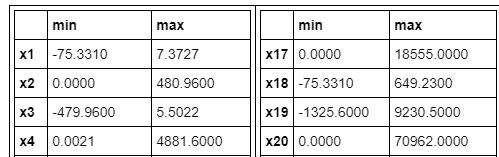
\includegraphics[scale = .6]{imgs/feature_range.JPG}
  \caption{A snippet for the range of each feature for Year 2 using \textbf{pandas'} describe function}
  \label{table:feature_range}
\end{table}
 